\begin{figure}[H]
\centering
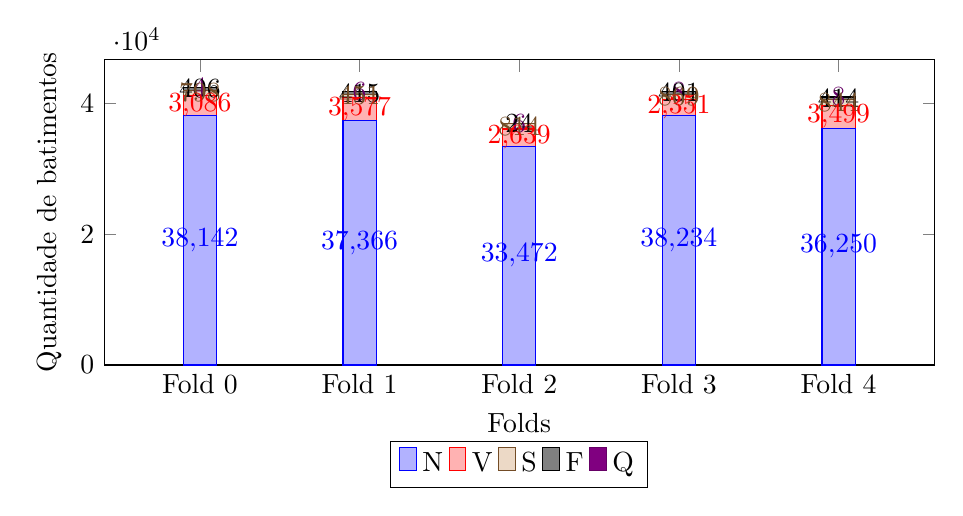
\begin{tikzpicture}
\begin{axis}[
    ybar stacked,
    bar width=12pt,
    width=\textwidth,
    height=0.45\textwidth,
    symbolic x coords={Fold 0,Fold 1,Fold 2,Fold 3,Fold 4},
    xtick=data,
    ylabel={Quantidade de batimentos},
    xlabel={Folds},
    legend style={at={(0.5,-0.25)}, anchor=north, legend columns=-1},
    nodes near coords,
    enlarge x limits=0.15,
    ymin=0
]

\addplot+[ybar] plot coordinates {(Fold 0,38142) (Fold 1,37366) (Fold 2,33472) (Fold 3,38234) (Fold 4,36250)};
\addplot+[ybar] plot coordinates {(Fold 0,3086) (Fold 1,3577) (Fold 2,2639) (Fold 3,2351) (Fold 4,3499)};
\addplot+[ybar] plot coordinates {(Fold 0,798) (Fold 1,451) (Fold 2,814) (Fold 3,869) (Fold 4,844)};
\addplot+[ybar] plot coordinates {(Fold 0,406) (Fold 1,415) (Fold 2,24) (Fold 3,401) (Fold 4,414)};
\addplot+[ybar] plot coordinates {(Fold 0,4) (Fold 1,6) (Fold 2,6) (Fold 3,8) (Fold 4,8)};

\legend{N, V, S, F, Q}
\end{axis}
\end{tikzpicture}
\caption{Distribuição de batimentos por tipo de arritmia em cada fold (treino).}
\label{fig:class_freq_all}
\end{figure}